% Chapter Template

\chapter{Using Correct by Construction with Agile Scrum} % Main chapter title

\label{CbyCWithAgileScrum} % Change X to a consecutive number; for referencing this chapter elsewhere, use \ref{ChapterX}

\section{Why not just Agile Scrum}

The driving force behind Agile Scrum is the ability to react to changing requirements.
To evaluate requested changes the changes have to be implemented. 
If we evaluate this against the Agile manifesto:
\begin{description}
	\item [Responding to change:]  In order to evaluate a change: a story has to be
		created, and the story has to be refined and sized. Then, depending on the 
		priority, existing work has to be moved to make resources available to implement
		the change. 
	\item [Working software:] We have to implement the requested change in order to
		validate it. If the requested change does not work we might end up with invalid or
		non-functional software. The changes then has to be rolled back.
	\item [Customer collaboration] For a change to be actioned the team will reason
		through it on a whiteboard. This reasoning is based on opinion and results in
		arguments that cannot be resolved without implementing the change.
\end{description}

\section{Augment Scrum with Correct by Construction}

The CbyC process is designed to validate changes at every step. By augmenting
Scrum with CbyC we reduce the need to implement a change before it can be validated.
Thereby streamlining the development process and reducing the risk of having broken or invalid software.
Figure \ref{fig:ScrumCbyCWorkflow} shows how the Scrum process can be augmented with CbyC.

\subsection{Roles}

\subsubsection{Team Architect}
We add the Team Architect to help the Product Owner create the Formal Specification.
This role can be shared amongst the team members and does not have to belong to a
specific person.

\subsection{Events}

\subsubsection{Product Planning}
In Scrum the Product Owner can create the Product Backlog without assistance
from the rest of the team. The Product Owner can still create the 
System Requirements Specification on his own, but the Formal Specification is
written in a mathematical language and the Product Owner might need help writing
it. To facilitate the writing of the System Requirements Specification and the 
Formal Specification we add the Product Planning event. During the Product Planning 
event the Team Architect helps the Product Owner write the Formal Specification.
Once a change has been added to the Formal Specification and verified, user 
stories can be added to the Product Backlog. Requirements should be traceable 
through the System Requirements Specification and Formal Specification to the story
in the Product Backlog.

\subsubsection{Sprint}
To the normal Sprint development work we add, from CbyC, the Formal Specification,
Formal Design, System Test Specification, and the INFORMED Design. The stories in
the Sprint Backlog tells us what work we are going to do to create the increment. We 
take the work described by the story and the specification in the Formal Specification 
and we then accordingly update the Formal Design, System Test Specification 
and INFORMED design. After verification we write the code to create/update the
Increment.

\subsection{Artefacts}

We add the artifacts as describe by CbyC: 

\begin{enumerate}
	\item System Requirements;
	\item Formal Specification;
	\item Formal Design;
	\item System Test Specification;
	\item INFORMED Design.
\end{enumerate}  

\subsubsection{Increment}
We create the Increment as described by CbyC Code Artifact.


\begin{figure}[H]
	\centering
	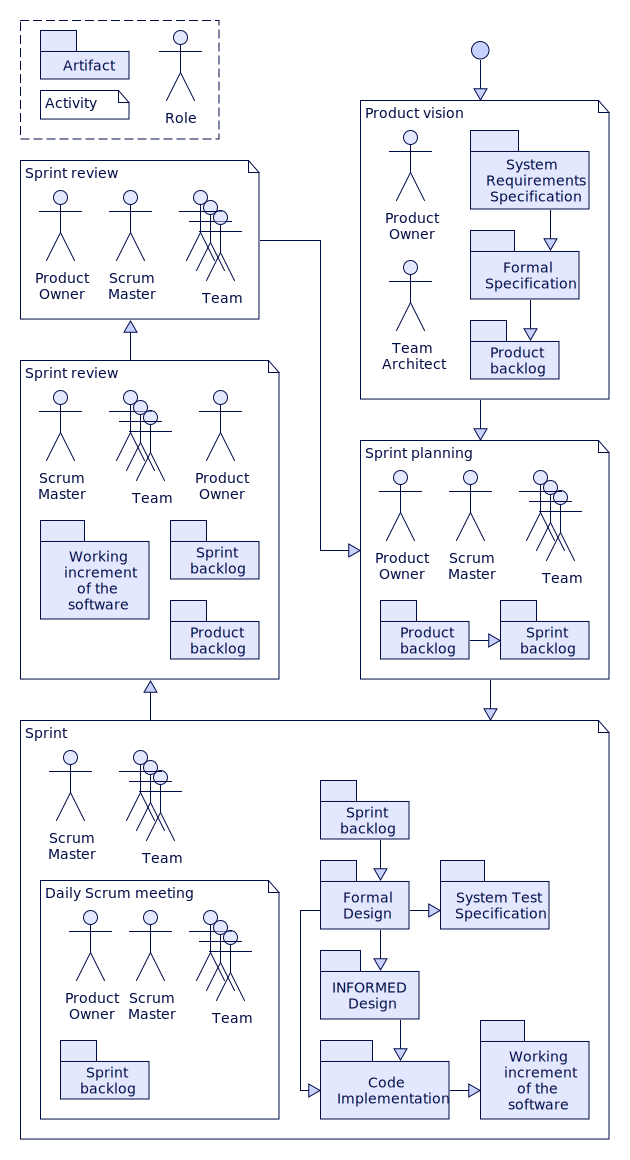
\includegraphics[scale=0.75]{Figures/Scrum_CbyC_workflow.pdf}
	\decoRule
	\caption{The Scrum workflow augmented with CbyC.}
	\label{fig:ScrumCbyCWorkflow}
\end{figure}